\documentclass[12pt]{article}
\usepackage[english]{babel}
\usepackage{natbib}
\usepackage{url}
\usepackage[utf8x]{inputenc}
\usepackage{amsmath}
\usepackage{graphicx}
\graphicspath{{images/}}
\usepackage{parskip}
\usepackage{fancyhdr}
\usepackage{vmargin}
\usepackage{tabularx}
\usepackage{xcolor}
\usepackage{listings}
\usepackage{xparse}
\usepackage{multirow}
\usepackage{booktabs}
\NewDocumentCommand{\codeword}{v}{%
\texttt{\textcolor{black}{#1}}%
}
\lstset{language=C,keywordstyle={\bfseries \color{black}}}

\setmarginsrb{2.5 cm}{2 cm}{2 cm}{2 cm}{1 cm}{1 cm}{1 cm}{1 cm}

\title{Assignment Report}								% Title
\author{Eric Leonardo Lim \\ Gede Bagus Bayu Pentium}	% Author
\date{\today}											% Date

\makeatletter
\let\thetitle\@title
\let\theauthor\@author
\let\thedate\@date
\makeatother

\pagestyle{fancy}
\fancyhf{}
\rhead{\theauthor}
\lhead{\thetitle}
\cfoot{\thepage}

\begin{document}

%%%%%%%%%%%%%%%%%%%%%%%%%%%%%%%%%%%%%%%%%%%%%%%%%%%%%%%%%%%%%%%%%%%%%%%%%%%%%%%%%%%%%%%%%

\begin{titlepage}
	\centering
    \vspace*{0.5 cm}
    
\includegraphics[scale = 2.7]{ntu.jpg}\\[1.0 cm]	% University Logo
    \textsc{\LARGE Nanyang Technological University}\\[2.0 cm]	% University Name
	\textsc{\Large CZ4013}\\[0.5 cm]				% Course Code
	\textsc{\large Distributed Systems}\\[0.5 cm]				% Course Name
	\rule{\linewidth}{0.2 mm} \\[0.4 cm]
	{ \huge \bfseries \thetitle}\\
	\rule{\linewidth}{0.2 mm} \\[1.5 cm]
	
	\begin{minipage}{0.4\textwidth}
		\begin{flushleft} \large
			\emph{Author:}\\
			\theauthor
			\end{flushleft}
			\end{minipage}~
			\begin{minipage}{0.4\textwidth}
			\begin{flushright} \large
			\emph{Matric. no.:} \\
			U1420158D\\
            U1420090G% Your Student Number
		\end{flushright}
	\end{minipage}\\[2 cm]
	
	{\large \thedate}\\[2 cm]
 
	\vfill
	
\end{titlepage}

%%%%%%%%%%%%%%%%%%%%%%%%%%%%%%%%%%%%%%%%%%%%%%%%%%%%%%%%%%%%%%%%%%%%%%%%%%%%%%%%%%%%%%%%%

\tableofcontents
\pagebreak

%%%%%%%%%%%%%%%%%%%%%%%%%%%%%%%%%%%%%%%%%%%%%%%%%%%%%%%%%%%%%%%%%%%%%%%%%%%%%%%%%%%%%%%%%

\section{Introduction}
This project consolidates basic knowledge about interprocess communication and remote invocation through constructing client and server programs that use UDP as the transport protocol. The client and server programs are designed to simulate a distributed banking system.

\subsection{Environment}
The following are the necessary environment to run the system.

\begin{itemize}
	\item \textbf{Operating System} --- The banking system is developed and tested in a GNU/Linux environment. 
    \item \textbf{Programming Language} --- There are two languages used to develop the system. The server is developed using \codeword{C++} and the client is developed using \codeword{Java}.
\end{itemize}

\subsection{Assumption}
Several assumptions have been made in developing the system, as follows:

\begin{itemize}
	\item \textbf{User Interface} --- The user interaction to the system is fully done in command-line interface (no Graphical User Interface).
	\item \textbf{User Input} --- There are minimum error checking in user input to the system. The system assume all the user input are valid.
    \item \textbf{Request Concurrency} --- Server and client are handling the user input in sequential order. The system assume only one request at a time is performed.
    \item \textbf{Client-Server Communication} --- All clients are assumed to know server address and port number.
    \item \textbf{Storage} --- This system does not have any persistent storage (All information are contained in memory).
\end{itemize}

\pagebreak
\section{Design}

\subsection{Architecture Design}
The system used UDP as communication protocol between client and server.
\begin{figure}[htbp!]
    \centering
    
\includegraphics[width=0.6\textwidth]{client-server.png}
    \caption[Client and Server]{Communication between client and server}
    \label{fig:client-server}
\end{figure} 

\subsubsection{Server}
The server architecture can be seen in Figure~\ref{fig:server-architecture}.
\begin{figure}[htbp!]
    \centering
    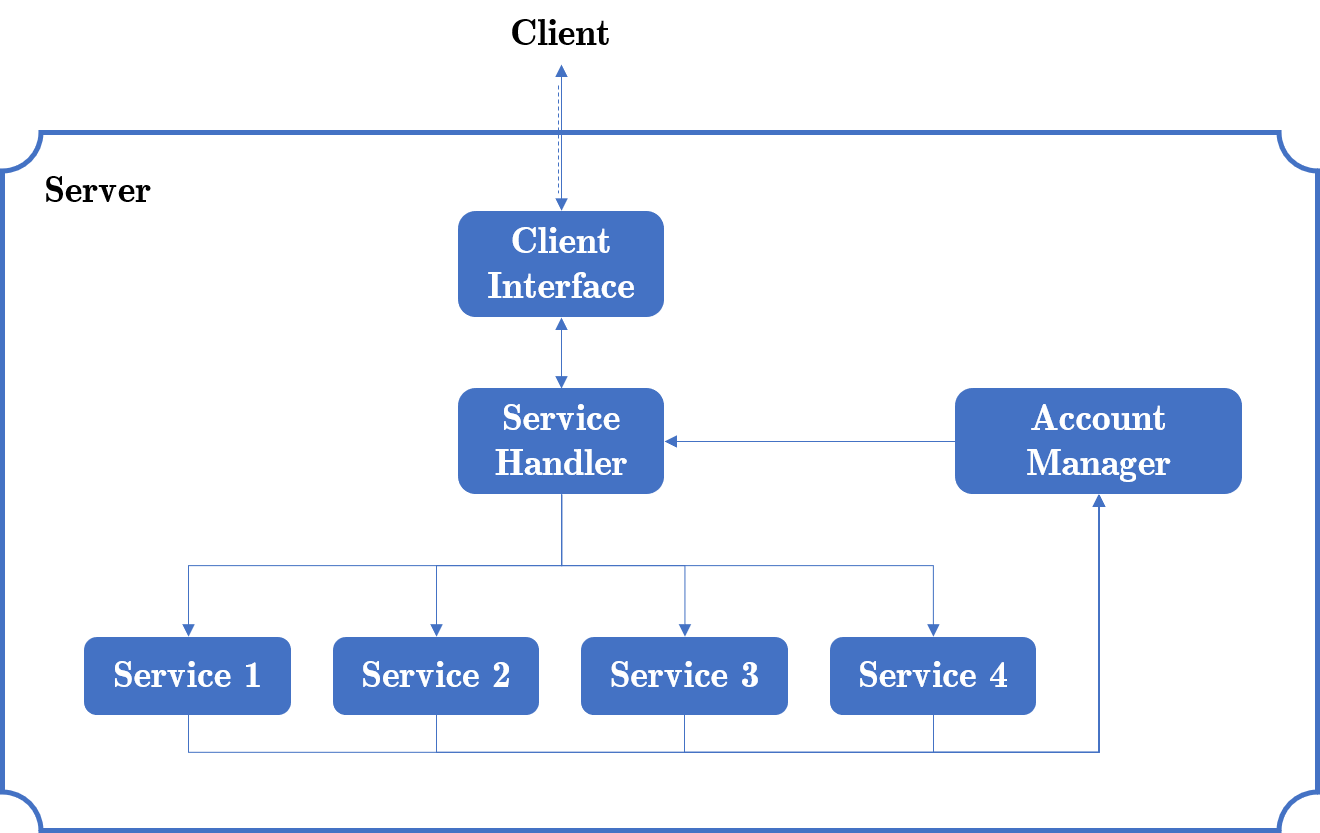
\includegraphics[width=1.0\textwidth]{server.png}
    \caption[Server Architecture]{Server architecture}
    \label{fig:server-architecture}
\end{figure}

\subsubsection{Client}
The client architecture can be seen in Figure~\ref{fig:client-architecture}
\begin{figure}[htbp!]
    \centering
    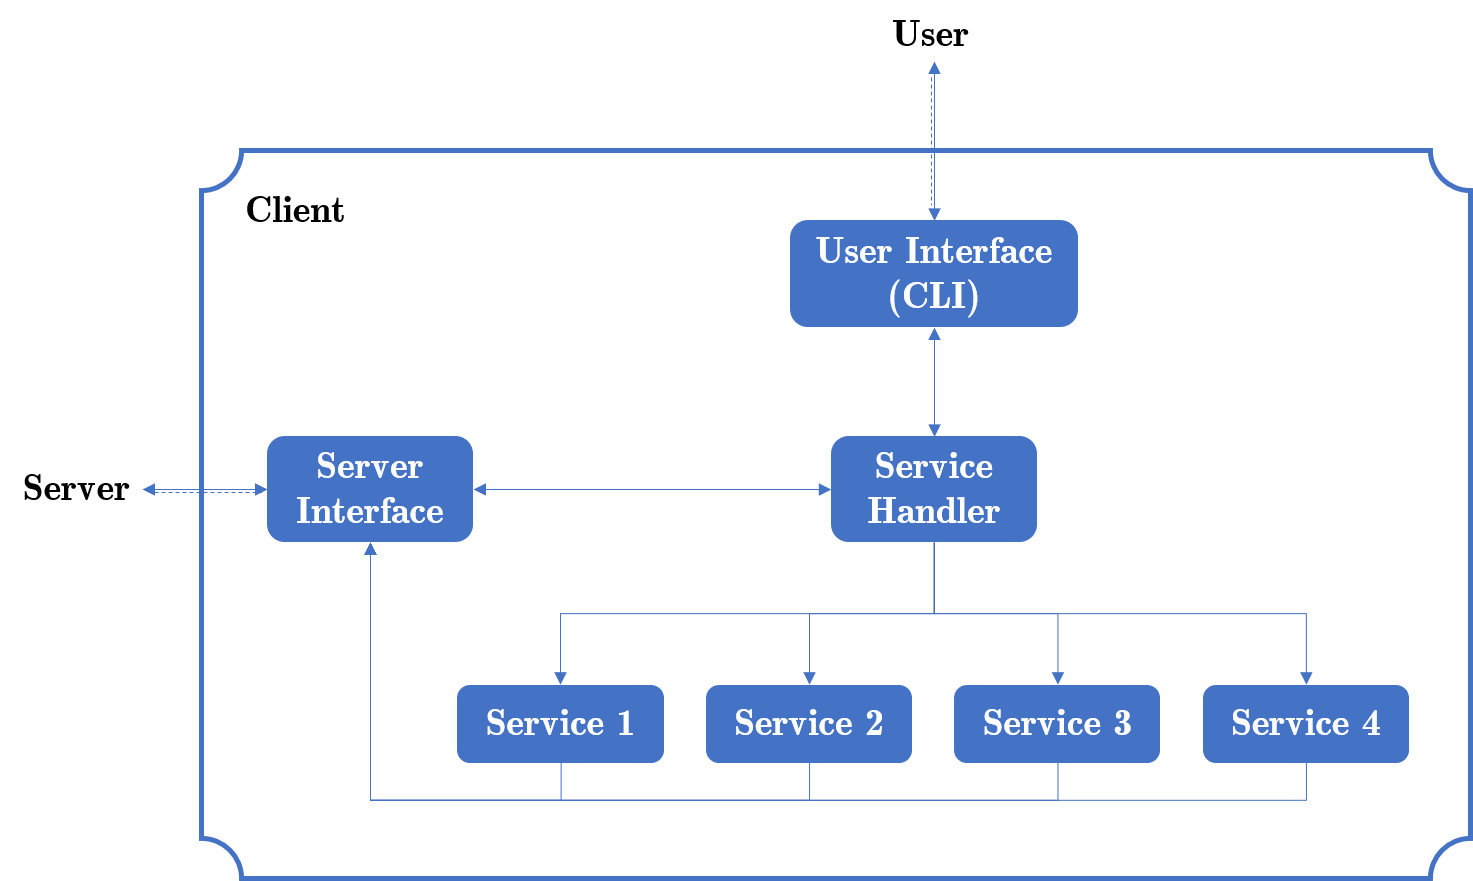
\includegraphics[width=1.0\textwidth]{client.png}
    \caption[Client Architecture]{Client architecture}
    \label{fig:client-architecture}
\end{figure}

\subsection{Communication Design}

\subsubsection{Message Structure}
Each message (request/response/acknowledgement) is performed with two transmissions, i.e. transmission of header followed by transmission of content.

The header size is constant, i.e. 4 bytes. It is an integer which represents the size of the actual content. This allows the recipient to adjust the buffer size for receiving the content.

The content message format varies on whether it is a request, response, or an acknowledgement. Generally, for request messages, the format is divided into sections, such as request ID and data, consecutively. For response messages, the format is divided into response ID, status, and data. For acknowledgement, it is divided into response ID and status.

The data section format depends on the service type. Each service type requires passing a message consisting of a few primitive data-types, such as integers, floating-point values, and strings. Each data to be passed is converted into byte-arrays and is prepended with the number of bytes required, and then concatenated into one, i.e. the data section of the message.

The structure for each service will be described in detail in Section \ref{services}.

\subsubsection{Marshalling/Unmarshalling Primitive Datatypes}

\paragraph{Integer values}
Since \codeword{int} is used in both server (C++) and client (Java) programs, integer values are represented in 4 bytes and is able to represent negative values.

Marshalling an integer into a byte array of size $4$ is as simple as obtaining each octet and then assigning the octet to the corresponding index in the byte array. Since in both C++ and Java, when assigning an \codeword{int} into a \codeword{byte}, only the last 8 bits of the integer will be captured, each octet in the integer can be obtained by right-shift operations. To obtain the $i^{th}$ octet, the integer is right-shifted $8\cdot(4-i)$ number of times.

Unmarshalling the byte array into an integer value can be achieved by performing left-shift operations on the values of each index $i$ of the byte array, with each value of index $i$ to be left-shifted $8\cdot(4-i)$ number of times, and then performing \codeword{OR} operations to combine them into one integer.

\paragraph{Floating-point values}
We are using \codeword{float} to represent all floating-point values in both sever and client programs, so each floating-point value is 32-bit. Since \codeword{float} in C++ is implemented in the same way as it is in Java , i.e. as 32-bit precision IEEE 754 floating points, we can perform marshalling and unmarshalling on floating-point values in the same way as doing so on integer values.

\paragraph{Enumerated type values}
We represent enumerated type values as integer values, so marshalling and unmarshalling is performed in exactly the same way.

\paragraph{Strings}
By employing the aforementioned message structure, both variable-length and fixed-length strings can be represented uniformly, i.e. only as byte-arrays with each byte representing each character.

\pagebreak
\section{Services}
\label{services}

\paragraph{Request}
The general format of all the request is:
\begin{itemize}
	\item \textit{ID} --- [\codeword{4 bytes}] request id generated by the client.
    \item \textit{Service type} --- [\codeword{4 bytes}] type of request send from the client.
    \item \textit{Header of Content 1} --- [\codeword{4 bytes}] header length of content 1.
    \item \textit{Content 1} --- [\codeword{Variable length}] content 1 of the request.
    \item \textit{Header of Content 2} --- [\codeword{4 bytes}] header length of content 2.
    \item \textit{Content 2} --- [\codeword{Variable length}] content 2 of the request.
    \item \dots
\end{itemize}

\paragraph{Response}
The general format of all the response is:
\begin{itemize}
	\item \textit{ID} --- [\codeword{4 bytes}] response id generated by the server.
    \item \textit{Status} --- [\codeword{1 byte}] response status
    \item \textit{Header of Content 1} --- [\codeword{4 bytes}] header length of content 1.
    \item \textit{Content 1} --- [\codeword{Variable length}] content 1 of the response.
    \item \textit{Header of Content 2} --- [\codeword{4 bytes}] header length of content 2.
    \item \textit{Content 2} --- [\codeword{Variable length}] content 2 of the response.
    \item \dots
\end{itemize}

\subsection{Service 1: Open New Account}
This service allows users to create a new account in the system by specifying \textit{name}, \textit{password}, \textit{default currency}, and \textit{initial balance}. If the request is successfully processed, the server replies with a response with the \textit{account number} assigned to the account.

The request message of this service has the following format:

\noindent\begin{minipage}{\linewidth}
	\centering
	\begin{tabular}{c l l}
  	\hline
    \textbf{Content} & \textbf{Parameter} & \textbf{Type}\\
    \hline
    1 & Name & Variable-length string \\
    2 & Password & Fixed-length String \\
    3 & Currency & Enumerate \\
    4 & Balance & Float \\
    \hline
	\end{tabular}
\end{minipage}

The response of this service has the following format:

\noindent\begin{minipage}{\linewidth}
	\centering
	\begin{tabular}{c l l}
  	\hline
    \textbf{Content} & \textbf{Parameter} & \textbf{Type}\\
    \hline
    1 & Account Number & Integer \\
    \hline
	\end{tabular}
\end{minipage}


\subsection{Service 2: Close Existing Account}
This service allows user to close an existing account in the system by specifying \textit{name}, \textit{account number}, and \textit{password}. If the request is successfully processed, the server response with acknowledgment.

The request of this service has the following format:

\noindent\begin{minipage}{\linewidth}
	\centering
	\begin{tabular}{c l l}
  	\hline
    \textbf{Content} & \textbf{Parameter} & \textbf{Type}\\
    \hline
    1 & Name & Variable-length string \\
    2 & Account Number & Integer \\
    3 & Password & Fixed-length string \\
    \hline
	\end{tabular}
\end{minipage}

The response of this service is only acknowledgment whether the service is successful or not. This acknowledgement is represented by the response status.

\subsection{Service 3: Deposit/Withdraw Money}
This service allows user to deposit or withdraw money to their account by specifying \textit{name}, \textit{account number}, \textit{password}, \textit{currency} and \textit{balance}. If the request is successfully processed. the server response with acknowledgment and remaining balance in the account.

The request of this service has the following format:

\noindent\begin{minipage}{\linewidth}
	\centering
	\centering
	\begin{tabular}{c l l}
    \hline
    \textbf{Content} & \textbf{Parameter} & \textbf{Type}\\
    \hline
    1 & Name & Variable-length string \\
    2 & Account Number & Integer \\
    3 & Password & Fixed-length string \\
    4 & Currency & Enumerate \\
    5 & Balance & Float \\
    \hline
	\end{tabular}
\end{minipage}

The response of this service has the following format:

\noindent\begin{minipage}{\linewidth}
	\centering
	\begin{tabular}{c l l}
  	\hline
    \textbf{Content} & \textbf{Parameter} & \textbf{Type}\\
    \hline
    1 & Currency & Enumerate \\
    2 & Updated Balance & Float \\
    \hline
	\end{tabular}
\end{minipage}

\subsection{Service 4: Monitor Update}
This service allows the user to monitor update in the system by specifying the \textit{duration} of the monitor in milliseconds. If the request is successfully processed, the server response with acknowledgment and subsequently sending a callback to the client for each update happens during the \textit{duration} specified.

The request of this service has the following format:

\noindent\begin{minipage}{\linewidth}
	\centering
	\begin{tabular}{c l l}
    \hline
    \textbf{Content} & \textbf{Parameter} & \textbf{Type}\\
    \hline
    1 & Duration & integer \\
    \hline
	\end{tabular}
\end{minipage}

The response of this service has the following format:

\noindent\begin{minipage}{\linewidth}
	\centering
	\begin{tabular}{c l l}
  	\hline
    \textbf{Content} & \textbf{Parameter} & \textbf{Type}\\
    \hline
    1 & Update & String \\
    \hline
	\end{tabular}
\end{minipage}

\subsection{Service 5: Change Password}
This service allows user to change password by specifying \textit{name}, \textit{account number}, \textit{old password}, and \textit{new password}. If the request is successfully processed, the server response with acknowledgment.

The request of this service has the following format:

\noindent\begin{minipage}{\linewidth}
	\centering
	\begin{tabular}{c l l}
    \hline
    \textbf{Content} & \textbf{Parameter} & \textbf{Type}\\
    \hline
    1 & Name & Variable-length string \\
    2 & Account Number & Integer \\
    3 & Old Password & Fixed-length string \\
    4 & New Password & Fixed-length string \\
    \hline
	\end{tabular}
\end{minipage}

The response of this service is only acknowledgment whether the service is successful or not. This acknowledgement is represented by the response status.

\subsection{Service 6: Transfer Money}
This service allows user to transfer money to another user by specifying \textit{name}, \textit{account number}, \textit{recipient name}, \textit{recipient account number},\textit{password}, \textit{currency}, and \textit{balance}. If the request is successfully processed, the server response with acknowledgment and remaining balance in the account.

The request of this service has the following format:

\noindent\begin{minipage}{\linewidth}
	\centering
	\begin{tabular}{c l l}
    \hline
    \textbf{Content} & \textbf{Parameter} & \textbf{Type}\\
    \hline
    1 & Name & Variable-length string \\
    2 & Account Number & Integer \\
    3 & Recipient Name & Variable-length string \\
    4 & Recipient Account Number & Integer \\
    5 & Password & Fixed-length string \\
    6 & Currency & Enumerate \\
    7 & Balance & Float \\
    \hline
	\end{tabular}
\end{minipage}

The response of this service has the following format:

\noindent\begin{minipage}{\linewidth}
	\centering
	\begin{tabular}{c l l}
  	\hline
    \textbf{Content} & \textbf{Parameter} & \textbf{Type}\\
    \hline
    1 & Currency & Enumerate \\
    2 & Updated Balance & Float \\
    \hline
	\end{tabular}
\end{minipage}


\pagebreak
\section{Fault Tolerance}
The UDP is an alternative communication protocol to TCP. It is mainly designed for low latency and loss tolerating connections. To achieve low latency, UDP has no handshaking dialogues, thus exposes the protocol to any unreliability. Hence, the application layer needs to perform fault tolerance to achieve reliable communication.

\subsection{Invocation Semantics}
There are three techniques to handle failures, such as request message retransmission, duplicate filtering, and method re-execution/reply retransmission. In this project, we observe two out of them, i.e. At-Least-Once and At-Most-Once invocation semantics.

\begin{figure}[htbp!]
    \centering
    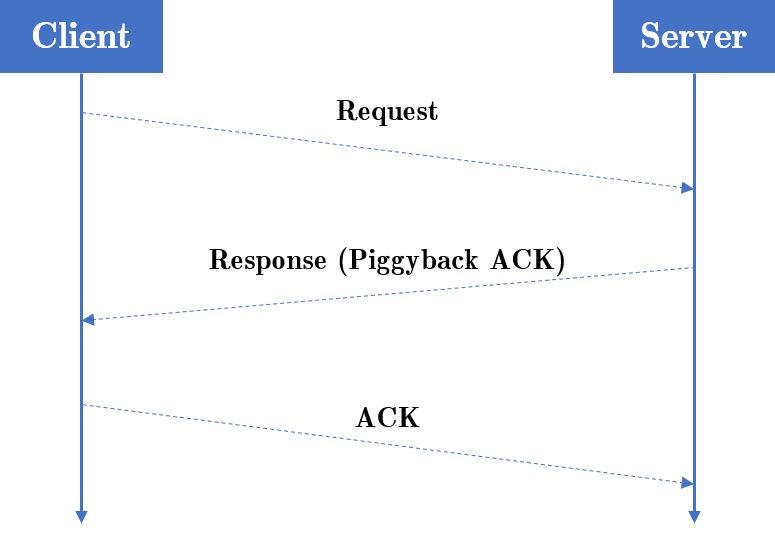
\includegraphics[width=0.6\textwidth]{handshake.png}
    \caption[Client-Server Handshake]{Client-server handshake}
    \label{fig:handshake}
\end{figure}


\subsubsection{At-Least-Once}
At-Least-Once semantic features request retransmission, but no duplicate filtering. Upon receiving duplicate messages, it cannot distinguish them as duplicates, so duplicate requests are handled by re-executing method. In our implementation, retransmission is performed whenever no reply is obtained within a particular period of time.

\subsubsection{At-Most-Once}
At-Most-Once semantic features request retransmission and duplicate filtering. Upon receiving duplicate messages, it resends the exact same reply that has already been sent before. In our implementation, message ID is used to distinguish whether two messages are duplicates. In case of server, the client address is also used in addition to the message ID. Upon the first time receiving a particular unique message as distinguished by the ID (and the client address, in case of server), the intended reply is saved.

\subsection{Comparison}

\subsubsection{Idempotent}

We use Service 5 to observe the fault tolerance of the two invocation semantics when handling idempotent operations. As illustrated in table \ref{table:idempotent_experiment}, the behaviors of the two invocation semantics when the response message failed to be sent to the client are alike, i.e. both are able to successfully handle the failures.

\begin{table}[htbp!]
    \centering
    \caption{Idempotent service fault tolerance result}
    \label{table:idempotent_experiment}
    \begin{tabularx}{\textwidth}{X l l}
        \toprule
        \multirow{2}{*}{\textbf{Fault}} & \multicolumn{2}{c}{\textbf{Invocation Semantic}} \\
        \cmidrule{2-3}
        & \textbf{At-Least-Once} & \textbf{At-Most-Once} \\ 
        \midrule
       	Request failure & client resends request  & client resends request \\ 
    	\hline
    	Response failure & password is successfully changed & password is successfully changed \\ 
    	\hline
    	Acknowledgement & server resends response & server resends response \\
        failure & client resends acknowledgment & client resends acknowledgment \\ 
        \bottomrule
    \end{tabularx}
\end{table}

\subsubsection{Non-Idempotent}
We use our service 6 to observe the fault tolerance of the two invocation semantics when handling non-idempotent operations. As illustrated in table \ref{table:nonidempotent_experiment}, the At-Least-Once invocation semantic produces an arbitrary failure, i.e. the transfer service is executed more than once. In contrast, the At-Most-Once invocation semantic is able to handle the failure successfully.

\begin{table}[htbp!]
    \centering
    \caption{Non-idempotent service fault tolerance result}
    \label{table:nonidempotent_experiment}
    \begin{tabularx}{\textwidth}{X l l}
        \toprule
        \multirow{2}{*}{\textbf{Fault}} & \multicolumn{2}{c}{\textbf{Invocation Semantic}} \\
        \cmidrule{2-3}
        & \textbf{At-Least-Once} & \textbf{At-Most-Once} \\ 
        \midrule
       	Request failure & client resends request  & client resends request \\ 
    	\hline
    	Response failure & transfer is executed more than once                                                              & transfer is executed once \\ 
    	\hline
    	Acknowledgement & server resends response & server resends response \\
        failure & client resends acknowledgment & client resends acknowledgment \\ 
        \bottomrule
    \end{tabularx}
\end{table}

\pagebreak
\section{Conclusion}

In this project, we have designed and implemented a distributed banking system using the client-server architecture that uses the UDP protocol to communicate between each other. We also experimented with how different invocation semantics affect fault-tolerance.

\end{document}
